\documentclass[12pt, a4paper]{article}
\usepackage[utf8]{inputenc} 
\usepackage[margin=1.1in]{geometry}
\usepackage{multicol}
\usepackage{multirow}
\usepackage{url}
\usepackage{graphicx}
\usepackage{amsfonts}
\usepackage[tbtags]{amsmath}
\usepackage{caption}
\usepackage{subcaption}
\usepackage[ruled,vlined,linesnumbered]{algorithm2e}
\usepackage{algpseudocode}

\title{
	\line(1,0){300}
	\endgraf\bigskip
	\Huge
	\begin{center}
		\emph{Vertex Cover Problem} \\
		\emph{\Large{Exact and Approximation Algorithms}}
		
	\end{center}
	\line(1,0){300}
	\bigskip
	\bigskip
}

\author{
	\large{Iftekhar Hakim Kaowsar}\\
	\large{Student ID : 1705045}\\\\
	\large{Apurba Saha}\\
	\large{Student ID : 1705056}\\\\\\\\
	\Large{Department of Computer Science and Engineering}\\
	\Large{Bangladesh University of Engineering and Technology}\\\\\\
}
\date{
	\endgraf\bigskip
	\Large{\today}
}
\begin{document}
	\maketitle
	\pagebreak
	\tableofcontents
	\pagebreak
	\section{Introduction}
	This report explains the well-known optimization problem Vertex Cover. In computer science, the problem of finding a minimum vertex cover is a classical optimization problem. In this report, we have shown two exact algorithms (one is brute-force and another is parameterized vertex cover). We have also shown an approximation algorithm for finding near optimal solution as we cannot use exact algorithms in real world problems.
	\section{Problem Definition}
	Suppose $G(V,E)$ is a graph, where $V$ is the set of vertices and $E$ is the set of edges.
	\textbf{Vertex Cover} of graph $G$ means a subset $V'\subseteq V$, so that for every edge $(u,v)$ $\epsilon$ $E$, either $u$ $\epsilon$ $V'$ or $v$ $\epsilon$ $V'$ or both are true. \\
	\textbf{Vertex Cover Problem} is about choosing the subset with minimum possible size, i.e. choosing $V'\subseteq V$ with minimum possible size where $V'$ is a vertex cover of $G$.
	\begin{figure}[h]
		\centering
		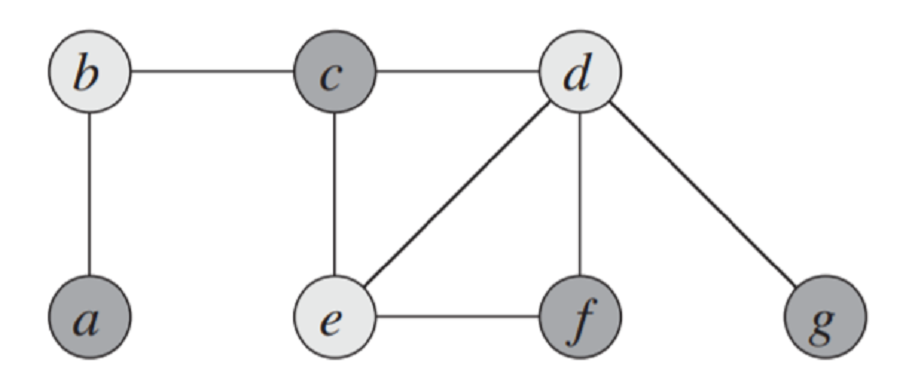
\includegraphics[scale=0.5]{intro_vc.PNG}
		\caption{\label{fig:intro_vc}Vertex Cover}
	\end{figure} \\
	From Figure \ref{fig:intro_vc}, vertices set $\{b, d, e\}$ comprises minimum vertex cover of the graph. However, set $\{a, c, e, f, g\}$ is another vertex cover, although it is not optimal. Again, set $\{a, b, c, f, g\}$ is not a vertex cover at all despite having a larger size than optimal set.
	\par
	A real world scenario of this problem can be described with an example of an area, where we need to set cameras to cover different roads. Graph edges will represent the roads and vertices will represent the end points. Now, finding minimum number of cameras is similar to vertex cover problem. Another example can be a museum site, where we need to set minimum number of guards.\\ \\
	\textbf{Decision version:} The decision version of the problem is about deciding whether a graph has a vertex cover of size at most $k$.
	If we can solve the decision version of the problem, we can solve the original problem (optimization version) too.
	\par
	Vertex cover problem is NP-complete. We do not expect a polynomial-time solution to solve it. This fact increases the weight of the problem.
	
	
	\pagebreak
	\section{Exact Algorithms}
	As we have already stated, there is no polynomial time solution known which can solve this problem. We can run a complete brute force to solve for a given graph. There are other algorithms too which just make optimizations to the complexity. We will analyze the brute force algorithm and the parameterized algorithm to solve the decision version of the problem.
	\subsection{Brute Force Algorithm}
	\subsubsection{Overview}
	From the problem description, the brute force algorithm for vertex cover problem is too obvious. Let us go through its details. \\
	Let the graph has $n$ vertices and we need to decide whether there is vertex cover of size at most $k$. If we can, we will also find the vertex cover set.\\
	The outline of the algorithm is ---
	\begin{itemize}
		\item If graph has more than $(n-1)k$ edges, return \textit{no} decision.
		\item Assume decision is \textit{no}.
		\item Check for each possible subset of the vertices with size at most $k$ as a vertex cover. If it is suitable, make the decision \textit{yes} and return this subset.
	\end{itemize}
	We observe that a selection of $k$ nodes can cover at most $(n-1)k$ edges. That is why, if graph has more than $(n-1)k$ edges, we can directly make our decision as \textit{no}.
	
	\subsubsection{Pseudocode}
	\begin{algorithm}[H]
		\SetAlgoLined
		\DontPrintSemicolon
		\KwIn{Graph $G$ and integer $k$}
		\KwOut{Returns vertex cover set if it exists}
		\If{$G.E.size > (n-1)k$ }
		{
			\Return “$no$”
		}
		\For{each  $U \subseteq G.V$ \textbf{with} $U.size \leq k$}
		{   \If {$U$ is vertex cover}
			{
				\Return $U$\;
			}
		}
		\Return “$no$”
		\caption{Brute-force  $VC(G, k)$}
	\end{algorithm}
	\pagebreak
	\subsubsection{Time Complexity}
	Let us assume adjacency list has been used to store the graph. Also, let $n$ is the number of vertices and $m$ is the number of edges. Now,
	\begin{itemize}
		\item Number of possible subset of size $k$ from a set of size $n$ is $\binom{n}{k}.$
		\item Testing whether a single subset covers the graph takes $O(m)$. We can rewrite it as $O(n k)$. Because if $m > (n-1) k$, there will never be a vertex cover of size $k$.
	\end{itemize}
	So, overall time complexity is $O\left(nk\binom{n}{k}\right) = O\left(kn^{k+1}\right)$.
	We note that it is exponential of $n$ or the number of vertices.
	\subsection{Parameterized Vertex Cover}
	\subsubsection{Overview}
	Now, we explore another algorithm which can solve our problem accurately. We call it \textit{Parameterized Vertex Cover (PVC)}. It will make a little improvement over the time complexity of brute-force algorithm. But it is still exponential. After analyzing it, we will make a comparison between brute-force algorithm and PVC. \\ \\
	Let $G(V,E)$ is a graph where $V$ is the set of vertices and $E$ is the set of edges. $(u,v)$ denotes an edge where $u$ and $v$ are the endpoints. We need to find out if there is a vertex cover of size at most $k$.\\
	\textbf{Key Observation}:\par If edge $e_1=(u,v)$ is an edge of graph $G$, any vertex cover must select at least one of $u$ and $v$. That means $u$ or $v$ must be one the selected $k$ vertices. \\
	Let us assume our final decision is \textit{yes} and we have vertex $u$ in our vertex cover set. This implies there is vertex cover of size at most $k-1$ in graph $G - u$. By term $G - u$, we mean the graph after excluding vertex $u$ and its incident edges from graph $G$. \par
	Without loss of generality, this observation is correct in case we have vertex $v$ in our vertex cover set. Hence, we get our recurrence relation.
	$$decision(G, k) = decision(G-u,k-1) \text{ or } decision(G-v,k-1)$$
	where $(u,v)$ is any edge of graph G.\\
	The base case is,
	$$decision(G,0) = 
	\begin{cases}
		true & \text{if G has no edge} \\
		false & \text{otherwise} \\
	\end{cases}
	$$
	Just like before, we can direct make our decision as \textit{no}, if graph has more than $(n-1)k$ edges at any moment. \\
	\begin{figure}[h]
		\centering
		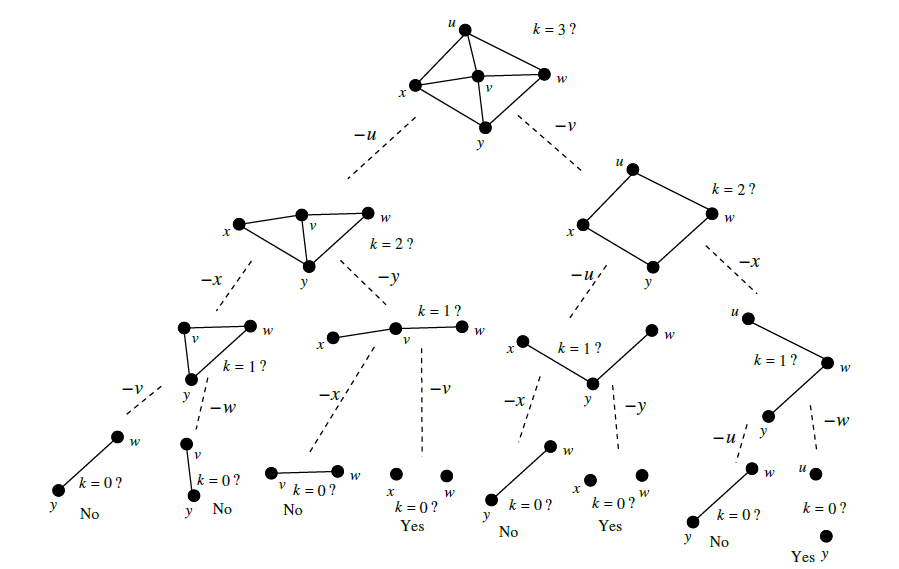
\includegraphics[scale=0.8]{pvc_sim.PNG}
		\caption{\label{fig:pvc}Parameterized Vertex Cover}
	\end{figure} \\
	Figure \ref{fig:pvc} shows recursion tree of PVC for an example graph. It is self-explanatory. Every time we break the graph by erasing a vertex. Once we reach the leaf level where our parameter or $k$ equals 0. If we can make \textit{yes} decision at a leaf, we can go upward to the root of recursion tree to get the vertex cover set. In Figure \ref{fig:pvc}, set $\{u, y, v\}$ or $\{v,x,w\}$ are the possible vertex cover set.
	\subsubsection{Pseudocode}
	\begin{algorithm}[H]
		\SetAlgoLined
		\DontPrintSemicolon
		\KwIn{Graph $G$ and integer $k$}
		\KwOut{Returns vertex cover set if it exists}
		\If{$G.E.size > (n-1)k$ }
		{
			\Return “$no$”
		}
		\If{$G.E.size = 0$}
		{
			\Return $\emptyset$
		}
		\If{$k=0$}{
			\Return “$no$”
		}
		$(u,v) \gets $ first element of $G.E$\; 
		\If{$PVC(G-u,k-1) \neq$ “$no$” }
		{
			$S \gets $ the return set of  $PVC(G-u,k-1)$\;
			\Return $S \cup u$
		}
		\If{$PVC(G-v,k-1) \neq$ “$no$” }
		{
			$S \gets $ the return set of  $PVC(G-v,k-1)$\;
			\Return $S \cup v$
		}
		\Return “$no$”\;
		\caption{Parameterized-Algorithm $PVC(G, k)$}
	\end{algorithm}
	
	\subsubsection{Time Complexity}
	To calculate $PVC(G,k)$, we recur to two branches, each requires rebuilding the adjacency list. Let $T(n,k)$ be the time required for $n$ vertices and parameter $k$. However, rebuilding the adjacency list takes $O(|E|)$ time, we can rewrite it as $constant \times kn$ , because $|E|\leq(n-1)k$ for \textit{yes} decision. We can solve the recurrence relation by iterative substitution method.
	\begin{align*}
		T(n,k) &\leq 2 T(n,k-1) + ckn \\
		&< 2\{2 T(n,k-2)+ckn\} +ckn \\
		&= 4 T(n,k-2) + 2 ckn + ckn \\
		&< 8 T(n,k-3) + 4 ckn + 2 ckn + ckn \\
		&= 2^3 T(n,k-3) + 2^2 ckn + 2^1 ckn + 2^0 ckn \\
		&< 2^k T(n,0) + 2^{k-1} ckn + 2^{k-2} ckn + ... +2^1 ckn + 2^0 ckn\\
		&< 2^k + 2^k ckn \\
		&= O(2^kkn)
	\end{align*}
	So, time complexity for the parameterized vertex cover problem is $O(2^kkn)$. \\
	We see it is still exponential, not feasible with a large graph. However, it is much better than the brute-force algorithm. Brute-force algorithm's time complexity includes exponential of $n$ or number of vertices, whereas PVC's time complexity includes exponential of $2$.
	\pagebreak
	\section{Approximation Algorithm}
	
	\subsection{Overview}
	Previously we have learned that vertex cover is an NP-complete problem. Even though (assuming \textbf{P $\neq$ NP} ) we
	can not hope for a polynomial time algorithm that always gets the best solution, we can develop
	polynomial time algorithms that produce a near optimal solution. In this section, we
	consider such an approximation algorithm for vertex cover problem. 
	
	
	The following approximation algorithm takes as input an undirected graph $G$ and returns a vertex cover whose size is guaranteed to be no more than twice the size
	of an optimal vertex cover.
	\begin{itemize}
		\item First we pick a random edge say,  ${\left(u,v\right)}$.
		\item We know any vertex cover must have at least one endpoint
		of it, so we take both endpoints.
		\item Then we throw out all edges incident to either ${u}$ or ${v}$.
		\item We keep repeating previous 3 steps
		until there are no uncovered edges left.
	\end{itemize}
	
	\subsection{Pseudocode}
	\begin{algorithm}[H]
		\SetAlgoLined
		\DontPrintSemicolon
		\KwIn{Graph $G$}
		\KwOut{Vertex cover set}
		${C = \emptyset}$\;
		${E' = G.E}$\;
		\While{${E' \neq \emptyset}$}{
			let, ${\left(u,v\right)}$ be an arbitrary edge of ${E'}$\;
			${C = C \cup \left\{u,v\right\}}$\;
			remove from ${E'}$ every edge incident to either ${u}$ or ${v}$\;
		}
		\Return ${C}$\;
		\caption{APPROX-VERTEX-COVER}
	\end{algorithm}
	
	~\newline
	\par The variable ${C}$ contains the vertex cover being constructed. Line $1$ initializes ${C}$ to the empty set. Line $2$ sets ${E'}$ to be a copy of the edge set ${G.E}$ of
	the graph. The loop of lines 3–7 repeatedly picks an edge ${\left(u,v\right)}$ from ${E'}$
	, adds its endpoints ${u}$ and ${v}$ to ${C}$, and deletes all edges in ${E'}$ that are covered by either ${u}$
	or ${v}$. Finally, line $8$ returns the vertex cover ${C}$.
	\pagebreak
	\begin{figure}[h]
		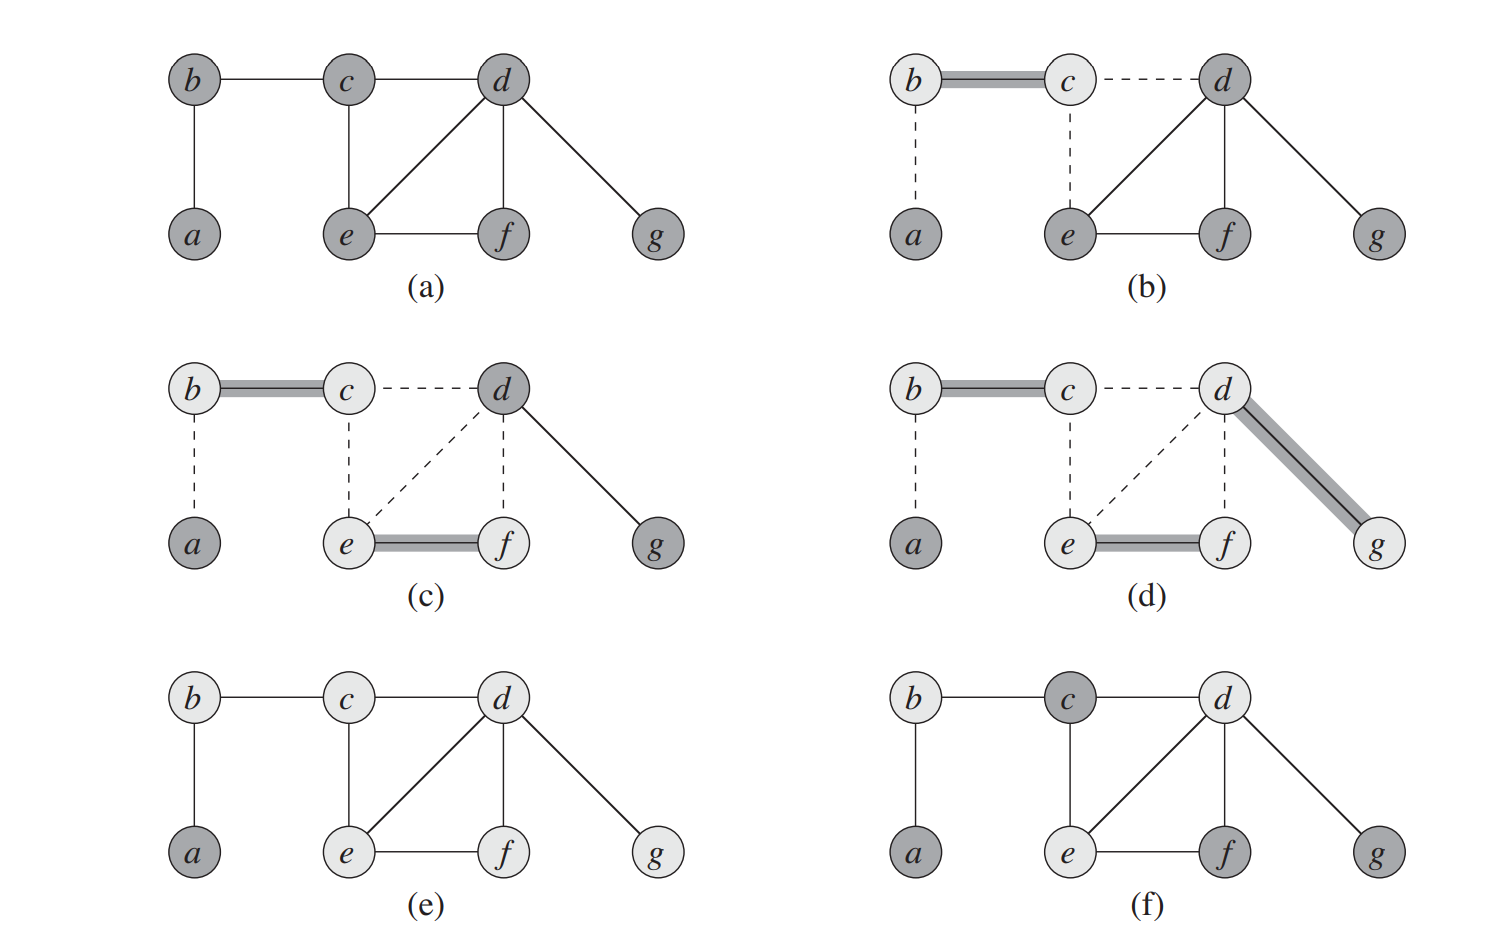
\includegraphics[width=1\textwidth]{ApproxGraph.png}
		\caption{The simulation of APPROX-VERTEX-COVER. \textbf{(a)} The input graph $G$ has seven
			vertices and eight edges. \textbf{(b)} The edge $\left(b,c\right)$, shown bold, is the first edge chosen by APPROX-VERTEX-COVER. Vertices $b$ and $c$, shown lightly shaded, are added to the vertex cover
			being created. Edges $\left(a,b\right)$, $\left(c,e\right)$, and $\left(c,d\right)$, shown dashed, are removed since they are now covered
			by some vertex in $C$. \textbf{(c)} Edge $\left(e,f\right)$ is chosen; vertices $e$ and $f$ are added to $C$. \textbf{(d)} Edge $\left(d,g\right)$
			is chosen; vertices $d$ and $g$ are added to $C$. \textbf{(e)} The set $C$, which is the vertex cover produced by
			APPROX-VERTEX-COVER, contains the six vertices $\left\{b, c, d, e, f, g\right\}$. \textbf{(f)} The optimal vertex cover for
			this problem contains only three vertices: $\left\{b, d, e\right\}$.}
	\end{figure}
	\pagebreak
	\subsection{Time Complexity}
	\begin{enumerate}
		\item If we consider adjacency lists to represent Graph ${G}$
		\begin{itemize}
			\item It takes ${O(1)}$ time to execute Line 1.
			\item Line 2 copies all the edges of the graph. So it takes ${O(|V| + |E|)}$ time to execute Line 2.
			\item From Line 3 to 7 we have a loop which runs until there are no edges left. So it takes ${O(|V| + |E|)}$ time to execute Line 3-7.
			\item Line 8 returns the answer. It takes ${O(|V|)}$ time to execute.
		\end{itemize} 
		So, the running time of this algorithm is ${O(|V| + |E|)}$
		
		\item If we consider adjacency matrix to represent Graph ${G}$
		\begin{itemize}
			\item It takes ${O(1)}$ time to execute Line 1.
			\item Line 2 copies all the edges of the graph. So it takes ${O\left(|V|^2\right)}$ time to execute Line 2.
			\item From Line 3 to 7 we have a loop which runs until there are no edges left. So it takes ${O\left(|V|^2\right)}$ time to execute Line 3-7.
			\item Line 8 returns the answer. It takes ${O(|V|)}$ time to execute.
		\end{itemize} 
		So, the running time of this algorithm is ${O\left(|V|^2\right)}$
	\end{enumerate}
	\subsection{Space Complexity}
	\begin{enumerate}
		\item The space complexity of this algorithm is ${O(|V| + |E|)}$ using adjacency list representation.
		\item The space complexity of this algorithm is ${O\left(|V|^2\right)}$ using adjacency matrix representation.
	\end{enumerate}
	
	\pagebreak
	
	
	\pagebreak
	\subsection{Proof of Factor 2 Approximation}
	\newtheorem{theorem}{Theorem}
	\begin{theorem}
		The APPROX-VERTEX-COVER is a polynomial time factor $2$ approximation algorithm.
	\end{theorem}
	\textbf{\textit{Proof.\\}}
	Let, \\\par${C}$ denote the set of vertices that is returned by APPROX-VERTEX-COVER\\
	\par${C^*}$ denote the set of vertices in the optimal vertex cover\\
	\par${K}$ denote the set of edges picked by APPROX-VERTEX-COVER\\\\
	\textbf{Key Observations}
	\begin{itemize}
		\item In the set of edges that were picked, no two share an endpoint.
		\item If the algorithm picked ${K}$ edges, the vertex cover found has size ${2K}$.
		
	\end{itemize}
	From these observations, any vertex cover must have size at least ${K}$ since
	it needs to have at least one endpoint of each of these edges. So, we have the lower
	bound
	
	\begin{equation}
		|{C^*}| ~~\geq~~ |{K}| \\
		\label{approxeqn:lower_bound}
	\end{equation}
	But, the vertex returned by the APPROX-VERTEX-COVER has size ${2K}$, yielding an exact upper bound on the size of the vertex cover returned
	\begin{equation}
		|{C}| ~~=~~ 2|{K}|\\
		\label{approxeqn:upper_bound}
	\end{equation}
	Combining Equations (\ref{approxeqn:lower_bound}) and (\ref{approxeqn:upper_bound}), we obtain
	\begin{equation}
		\begin{split}
			|{C}| ~~&=~~ 2|{K}|\\
			&\leq ~~2|{C^*}|
		\end{split}
	\end{equation}
	thereby proving the theorem.\\\\
	\textbf{Interesting fact:} Nobody knows any algorithm with approximation ratio $1.9$. 
	Best known is $2 - O\left(\frac{1}{\sqrt{\log n}}\right)$.
	\pagebreak
	\section{Comparison}
	Below we show some graphs and compare the result of exact algorithm with approximation algorithm.
	\begin{figure}[h]
		\begin{subfigure}[t]{.3\linewidth}
			\centering
			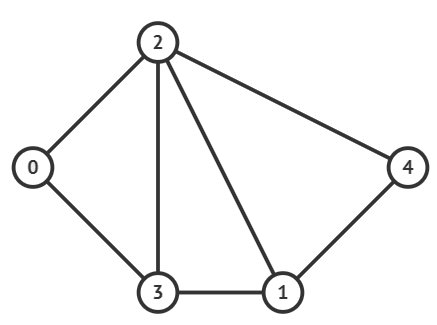
\includegraphics[width=.8\linewidth]{G1.png}
			\caption{Graph 1}
		\end{subfigure}
		\begin{subfigure}[t]{.3\linewidth}
			\centering
			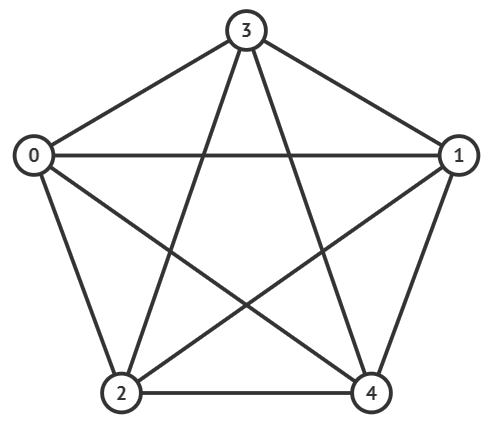
\includegraphics[width=.8\linewidth]{G2.png}
			\caption{Graph 2}
		\end{subfigure}
		\begin{subfigure}[t]{.3\linewidth}
			\centering
			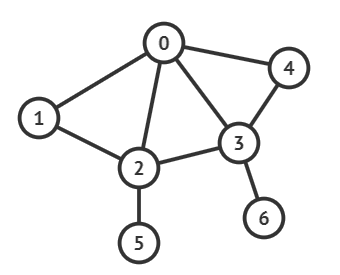
\includegraphics[width=.8\linewidth]{G4.png}
			\caption{Graph 3}
		\end{subfigure}
		\begin{subfigure}[t]{.5\linewidth}
			\centering
			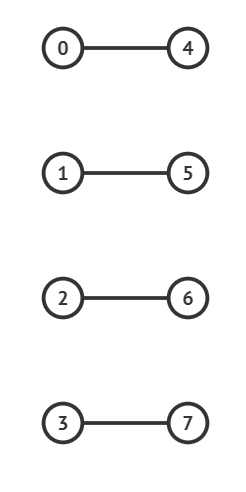
\includegraphics[scale=0.4]{G3.png}
			\caption{Graph 4}
		\end{subfigure}
		\begin{subfigure}[t]{.5\linewidth}
			\centering
			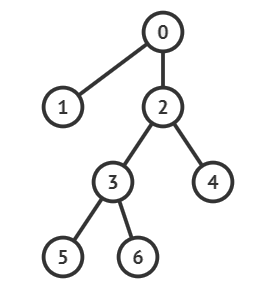
\includegraphics[scale=0.6]{G6.png}
			\caption{Graph 5}
		\end{subfigure}
		\begin{subfigure}[t]{1\linewidth}
			\centering
			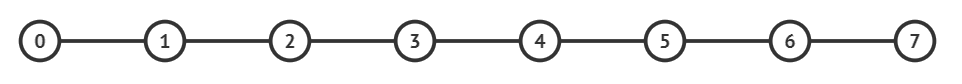
\includegraphics[scale=0.6]{G5.png}
			\caption{Graph 6}
		\end{subfigure}
	\end{figure}
	\begin{table}[h]
		\centering
		\begin{tabular}{|c|c|c|c|c|}
			\hline
			\multirow{2}{*}{Graph No.} & \multicolumn{2}{|c|}{Exact Algorithm} & \multicolumn{2}{|c|}{Approximation Algorithm}\\
			\cline{2-5}
			& Probable Vertex Cover & Cost & Probable Vertex Cover & Probable Cost\\
			\hline
			1 & $\left\{0,1,2\right\}$ & $3$ & $\left\{0,1,2,3\right\}$ & $4$\\
			\hline
			2 & $\left\{0,1,2,3\right\}$ & $4$ & $\left\{0,1,2,3\right\}$ & $4$\\
			\hline
			3 & $\left\{0,2,3\right\}$ & $3$ & $\left\{0,1,2,3\right\}$ & $4$\\
			\hline
			4 & $\left\{0,1,2,3\right\}$ & $4$ & $\left\{0,1,2,3,4,5,6,7\right\}$ & $8$\\
			\hline
			5 & $\left\{0,2,3\right\}$ & $3$ & $\left\{0,1,2,3\right\}$ & $4$\\
			\hline
			6 & $\left\{0,2,4,6\right\}$ & $4$ & $\left\{0,1,2,3,4,5,6,7\right\}$ & $8$\\
			\hline
		\end{tabular}
	\end{table}
	\pagebreak
	\section{Room for Improvement}
	For bipartite graphs, the result from approximation algorithm is almost twice for most of the cases. There is a room for improvement in case of bipartite graphs. Kőnig's theorem states that, in any bipartite graph, the minimum vertex cover set and the maximum matching set have in fact the same size. So if we are given a bipartite graph we can solve the maximum matching problem in that graph to determine the minimum vertex cover. Maximum matching can be done in $O\left(|V| \sqrt{|E|}\right)$ time using Hopcroft–Karp algorithm.
	
	For general graphs, we can increase the number of iteration to get a better result.
	\section{Conclusion}
	Vertex cover optimization serves as a model for many real-world and theoretical problems. The problem has been used to model the elimination of repetitive DNA sequences for synthetic biology and metabolic engineering applications. But whether or not it can be solved in polynomial time is still a question of interest.
\end{document}

